\documentclass{article}
\usepackage[utf8]{inputenc}
\usepackage{times}
\usepackage[titletoc]{appendix}
\usepackage{graphicx}
\usepackage{lineno}
\usepackage{multirow}
\usepackage[english]{babel}
\usepackage{typearea} 
\usepackage{amssymb}
\usepackage{amsfonts}
\usepackage{amsmath}
\usepackage{enumerate}
\usepackage{mathtools}
\usepackage{graphicx}
\usepackage{wrapfig}
\usepackage{lscape}
\usepackage{rotating}
\usepackage[colorinlistoftodos]{todonotes}
\newcommand{\Fig}[1]{Figure~\ref{fig:#1}}

\renewcommand{\baselinestretch}{1.5}
\newcommand{\bbar}[1]{\overline{#1}}

\newcommand\scalemath[2]{\scalebox{#1}{\mbox{\ensuremath{\displaystyle #2}}}}
\renewcommand{\familydefault}{\sfdefault}

\usepackage[font={small},labelfont={bf},justification=justified,margin=0.5cm]{caption}

\renewcommand{\thesection}{}
\renewcommand{\thesubsection}{\arabic{section}.\arabic{subsection}}

\usepackage{color}
	 \definecolor{darkred}{rgb}{0.9,0,0}
%	 \definecolor{darkgreen}{rgb}{0,0.5,0}
	 \definecolor{darkblue}{rgb}{0,0,0.75}
%	 \definecolor{magenta}{rgb}{0,0,0.75}
\newcommand{\hhone}{(H,H,1)}
\newcommand{\hhtwo}{(H,H,2)}
\newcommand{\hsone}{(H,S,1)}
\newcommand{\hstwo}{(H,S,2)}
\newcommand{\shone}{(S,H,1)}
\newcommand{\shtwo}{(S,H,2)}
\newcommand{\ssone}{(S,S,1)}
\newcommand{\sstwo}{(S,S,2)}

\newcommand{\hhstar}{(H,H,$\star$)}


\usepackage{hyperref}
\definecolor{darkgreen}{rgb}{0.1,0.6,0.3}
\definecolor{darkred}{rgb}{0.6,0.3,0.1}
\hypersetup{
    colorlinks=true,       % false: boxed links; true: colored links
    linkcolor=blue,          % color of internal links (change box color with linkbordercolor)
    citecolor=darkgreen,        % color of links to bibliography
    filecolor=magenta,      % color of file links
    urlcolor= black           % color of external links
}


% remove this before we submit...
\definecolor{greenie}{rgb}{0.1,0.62,0.0}
\definecolor{orange}{rgb}{0.9,0.3,0.0}
\definecolor{deepblue}{rgb}{0.0,0.0,0.7}
\newcommand{\marcus}[1]{{\color{orange}{#1}}}
\newcommand{\chaitanya}[1]{{\color{greenie}{#1}}}
\newcommand{\cha}[1]{\textcolor{darkgreen}{(#1)}}
\newcommand{\joe}[1]{{\color{deepblue}{#1}}}

\title{\vspace*{-22mm}\bf Title}
%\author{Chaitanya S. Gokhale$^{1}$, Joseph Bulbulia$^{2,3}$, Marcus Frean$^{4}$\\
%\normalsize $^1$Research Group for Theoretical Models of Eco-evolutionary Dynamics\\
%\normalsize Department of Evolutionary Theory, \\
%\normalsize Max-Planck Institute for Evolutionary Biology, 24306 Pl\"{o}n, Germany, \\
%\normalsize $^2$School of Humanities, Faculty of Arts, University of Auckland, New Zealand \\
%\normalsize $^3$Max Planck Institute for the Science of Human History, Jena, Germany \\
%\normalsize $^4$School of Engineering and Computer Science, \\
%\normalsize Victoria University of Wellington, New Zealand
%}


\date{}

\begin{document}

\linenumbers
\maketitle

\begin{abstract}
% Suggest we set this up differently:
Abstract stuff
\end{abstract}


\noindent
Keywords: social evolution, culture, narratives, stag-hunt


%\tableofcontents

\section{Introduction}
gwbniwbwnijb
\cite{skyrms:book:2003}

%\textbf{Collective cooperation and resource dynamics}.
%

\section{The dynamics stag hunt}

Replicator dynamics is the core idea of evolutionary dynamics. Replicator dynamics determines how the frequency of different strategies in a population changes over time.
We can analyze the equation used to determine replicator dynamics mathematically.
Let's take the frequency of $a$ and $b$ strategies are $x_a$ and $x_b$ and the fitness of each strategy is $f_a$ and $f_b$. It is a two-player game so we can say, $ x_a+x_b=1 $. We can write two differential equations using the above information
\[
{dx_a}/{dt} = x_a(f_a - \bar{f})    (1)
\] 
\[{dx_b}/{dt}= y(f_b - \bar{f})   (2)
\].
Now to keep the average fitness of the population constant, we can write an equation,
\[\bar{f}= (x_af_a+x_bf_b)   (3) \],
also, we can write the previously mentioned equation as $x_b=1-x_a$.
Now, we can substitute this $x_b$ value into the $3$ numbered equation, after substituting, we get the undermentioned equation.
\[\bar{f}={x_af_a+ (1-x_a)f_b} (4) \]
Now let's substitute the $(4)$ numbered equation into the $(1)$ equation
\[ dx_a/dt=x_a[f_a-(x_af_a+(1-x_a)f_b)]
          =x_a[f_a-x_af_a-f_b+x_af_b]
          =x_a[(1-x_a)f_a-(1-x_a)f_b]
          =x_a(1-x_a)(f_a-f_b) \] .
This is for a two-player population. If we have $n$ population, we can denote the equation of replicator dynamics as,
\[dx_i/dt=x_i[f_i(x)-\bar{f}]\]
where $i=1,2,3.....(n-1)$

To proceed with the replicator dynamics, we must understand simplex as the next step.
Simplex is a tool in evolutionary dynamics that helps us understand and visualize how a system evolved through an evolutionary process. We can denote this for $(n-1)$ strategies. But for simplicity, we took a two-player ($n=2$) homogenous process in which for $a$, $x_a=1$ and $x_b=0$, or the same goes for $b$, where, $x_a=0$ and $x_b=1$.
It will represent a line between points $a$ and $b$, with the midpoint being $x_a=x_b=0.5$. 
For another example, if we homogeneously use $ n=3$, it will represent an equatorial triangle, and the midpoint of the simplex will be $x_a=x_b=x_c=1/3$.
In population genetics, this simplex is known as the de Finetti diagram.
Let's get back to the replicator dynamics now,
\[dx_a/dt=x_a(1-x_a)(f_a-f_b)\],
What does this equation tell us? 
We can understand that the rate of change of the frequency of a certain type with time depends on the fitness, average fitness of the population, and frequency. From this understanding, we can state that if $f_i(x)-\bar{f}>0$ then the frequency of this type will increase over time, and if $f_i(x)-\bar{f}<0$, the frequency of the type will decrease over time.
If we make the change of strategy $a$ over time constant, which means $dx_a/dt=0$ then we can write the replicator dynamics equation as,
\[x_a(1-x_a)(f_a-f_b)=0\]
Now, if we try to find the certain under which $dx_a/dt$ will be $0$.
We will have three certain conditions,
\[x=0,x=1\] and \[f_a=f_b\]
$x=0$ and $x=1$ will be the two end points of a single line simplex and the joining point for the frequency graph and the dynamics of this frequency depends on the values of $f_a$ and $f_b$. If $f_a>f_b$ then the curve will be over the $0$ if $f_a<f_b$ then the curve will be under $0$, and for the condition $f_a=f_b$, it will make a straight line between the $0$ and $1$.For a visual representation of this graph, we can plot this equation for different values of $f_a$ and $f_b$ using Python.
\begin{figure}[h]
        \centering
        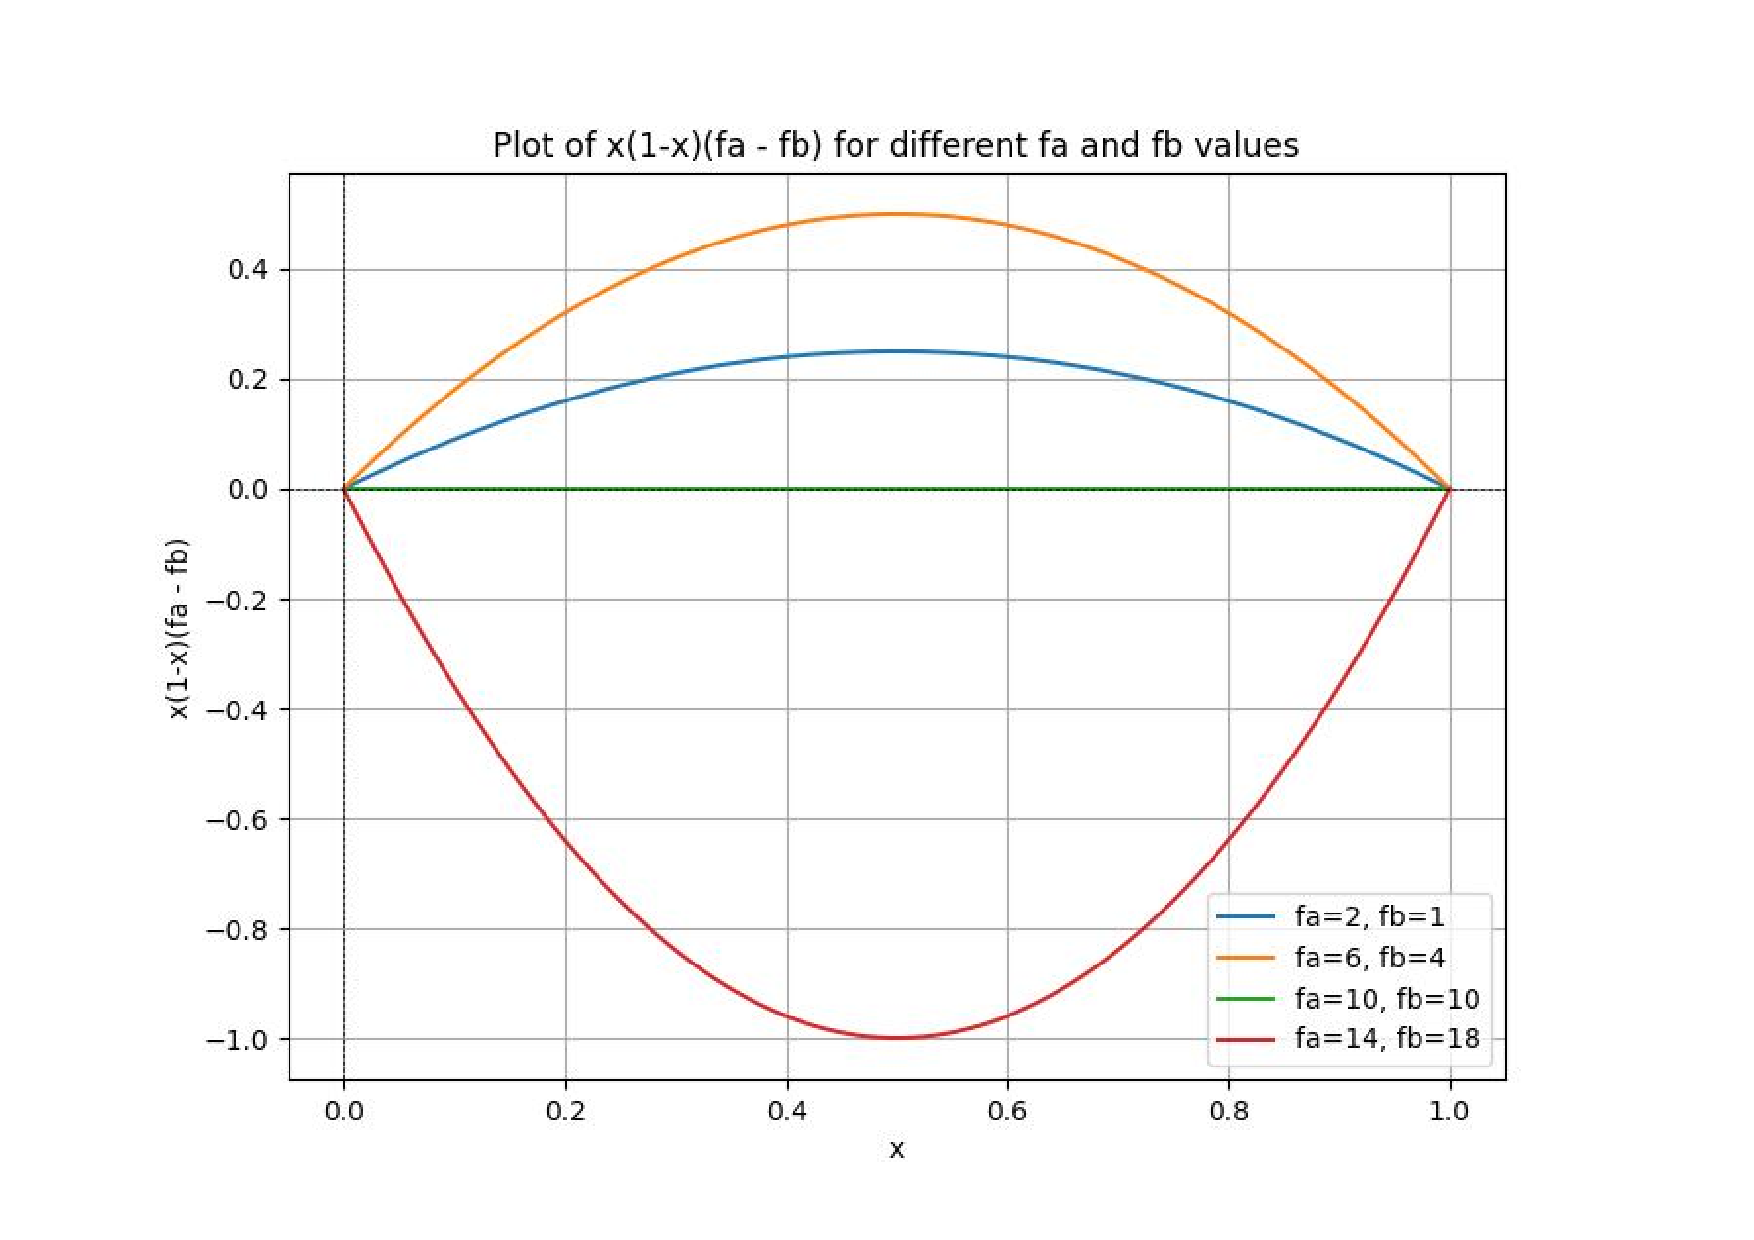
\includegraphics[width=0.5\linewidth]{Figure_1.png}
        \label{fig:Visualization of $x_a(1-x_a)(f_a-f_b)=0$}
    \end{figure}
We can get different conditions from this equation and graph. 
(1) Dominance: Where any of the two strategies will be dominant over another, means, for example if $f_a>f_b$ then strategy $a$ will be dominant over strategy $b$. It will be possible if the $a_1>b_1$ and $a_0>b_0$ where $a_1,a_0,b_1,b_0$ are the payoffs of a payoff matrix of a two-player game.
(2) Co-existence: It happens when one of the two strategies is rare and has an advantage for that. For example, if strategy $a$ is rare, then $f_a>f_b$ if $a$ becomes abundant, it will lose its advantage, so the inequality will be  $f_a<f_b$ and there will be a saturation point while becoming abundant from rare when the equation will $f_a=f_b$. In this scenario, the player should play the rare strategy.
(3) Bi-stability: A condition where all $a$ and $b$ will be stable means a strategy will get an advantage if it is abundant. For example, if strategy $a$ is abundant then the inequality will be $f_a>f_b$ and if it becomes rare then the inequality will be $f_a<f_b$ and there will be a saturation point when $f_a=f_b$. For this condition, the player should play the strategy that its opponent is playing.
(4) Neutrality: Now we have one condition in which both strategies will have the same impact. It does not depend on the change on the strategy. The equation for this strategy will be $f_a=f_b$. We mentioned this neutrality condition as saturation point before.
        
\section{Discussion}


\textbf{Code availability}.
Appropriate  computer code describing the model is available at 
\texttt{ REDACTED for review}.% {\url{https://github.com/tecoevo/beliefs}}.

\section{Acknowledgements}
\texttt{ REDACTED for review}.% {\url{https://github.com/tecoevo/beliefs}}.


\bibliographystyle{naturemag}
\bibliography{et.bib}

\renewcommand{\theequation}{SI.\arabic{equation}}
\setcounter{equation}{0}

\renewcommand{\thefigure}{SI.\arabic{figure}}
\setcounter{figure}{0}

\section{Supplementary material}


\subsection{Analysis of the simple system}

\bibliography{et.bib}


\end{document}
